\section{Marco Teórico} \label{sec:marcoteorico}
MPU6050: es una unidad de medida inercial o IMU de 6
grados de libertad, ya que combina un acelerómetro de 3 ejes
y un giroscopio de 3 ejes. Este sensor es ampliamente utilizado en
navegación, goniometría, estabilización, etc.

Acelerómetro: es un dispositivo que mide la vibración o
La aceleración del movimiento de una estructura.

Giroscopio: es un dispositivo mecánico utilizado para medir,
mantener o cambiar la orientación en el espacio de algunos
electrodoméstico o vehículo. 
\begin{figure}[htbp]
\centering
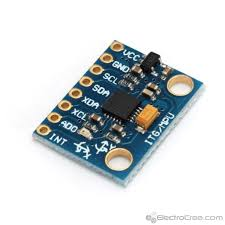
\includegraphics[width=5cm]{Figuras/acelerometro}
\caption{MPU6050 (Acelerometro y Giroscopio)}
\label{fig:acelerometro}
\end{figure}

Raspberry PI: es una placa computadora (SBC) de bajo coste, se podría decir que es un ordenador de tamaño reducido, del orden de una tarjeta de crédito, desarrollado en el Reino Unido por la Fundación Raspberry PI (Universidad de Cambridge) en 2011, con el objetivo de estimular la enseñanza de la informática en las escuelas, aunque no empezó su comercialización hasta el año 2012. \cite{vujovic2015raspberry}

\begin{figure}[htbp]
\centering
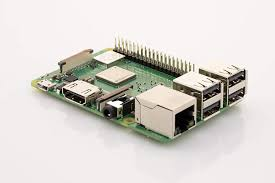
\includegraphics[width=5cm]{Figuras/rapsberry}
\caption{Rapsberry PI}
\label{fig:rapsberry}
\end{figure}

Puerto serie: es un módulo de comunicación digital para
un sistema integrado, es decir, permite la comunicación entre
Dos dispositivos digitales. Tiene dos conexiones, RX y
TX. Lo que indica los modos de comunicación que pueden
manejar, Full-duplex, Duplex y Simplex.

Sensibilidad: se refiere a la respuesta que el instrumento
la medición tiene que medir una variable y qué tan rápido es
esto para estabilizar su medida. 

VNC: Computación de red virtual. Es un programa de software gratuito basado en una estructura cliente-servidor que permite
observar las acciones de la computadora del servidor de forma remota para a través de una computadora cliente \cite{velasquez2013monitoreo}.

I2C: es un puerto y protocolo de comunicación serial, define
trama de datos y conexiones físicas para transferir bits
entre 2 dispositivos digitales. El puerto incluye dos cables.
comunicación, SDA y SCL. Además el protocolo permite
conecta hasta 127 dispositivos esclavos a esas dos líneas,
con velocidades de hasta 100, 400 y 1000 kbits / s.
\begin{figure}[htbp]
\centering
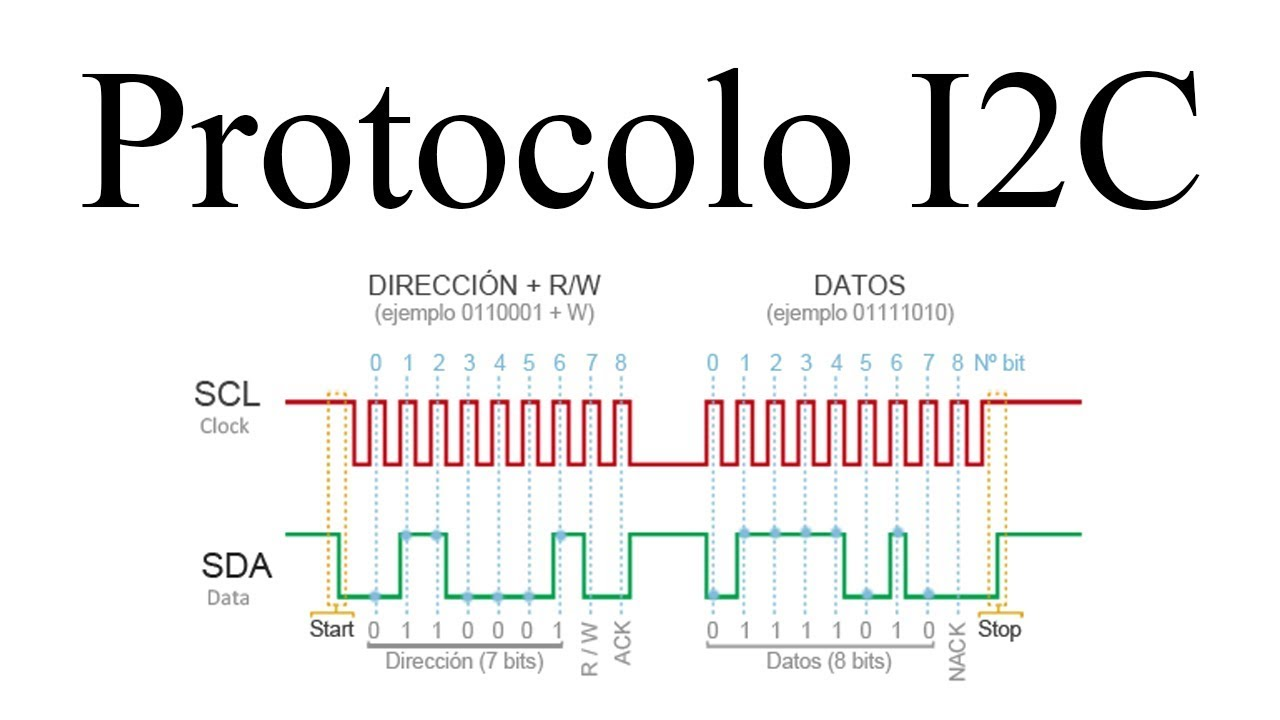
\includegraphics[width=7cm]{Figuras/I2C}
\caption{Protocolo I2C}
\label{fig:I2C}
\end{figure}



